\begin{figure}[ht]
  \begin{displaymath}
    \arraycolsep=0.9\cellsize
    \begin{array}{ccc}
      \nulltab{
        \\
        \put(4,0){\line(0,1){8}} \\
        \put(4,0){\line(0,1){8}} \\
        \put(4,0){\line(0,1){8}} \\
        \put(4,0){\line(0,1){8}} \\
        \put(4,0){\line(0,1){8}} \\
      }
      \nulltab{
        \usebox3 \put(-8,0){\line(1,0){8}} \\
        \usebox3 \put(-8,0){\line(1,0){8}} \\
        \usebox3 \put(-8,0){\line(1,0){8}} \\
        \cball \\
        \usebox3 \put(-8,0){\line(1,0){8}} \\
        \cball \put(-8,0){\line(1,0){8}} \\
      }
      \boxtab{ 
        
        \put(-4,-6.5){\line(1,0){8}} & \put(-4,-6.5){\line(1,0){8}} & \usebox3 & \usebox3 & & & \cball & & \\
        \put(-4,-6.5){\line(1,0){8}} & \put(-4,-6.5){\line(1,0){8}} & \put(0,0){\line(0,1){8}} \usebox3 & \cball & & & & \\
        \put(-4,-6.5){\line(1,0){8}} & \put(-4,-6.5){\line(1,0){8}} & \put(0,0){\line(0,1){8}} \usebox3 & \usebox3 & & \usebox3 & \cball & \\
        & b & \put(-4,0){\line(0,1){8}} & & \\
        \put(-4,-6.5){\line(1,0){8}} & \usebox3 & \put(0,0){\line(0,1){8}} \usebox3 & \cball & \\ 
        a & \put(-4,0){\line(0,1){8}} & \put(-4,0){\line(0,1){8}} \\\hline }
      
    \end{array}
  \end{displaymath}
  \caption{\label{fig:ecg_main}The main diagram showing the empty cell gap rule is satisfied.}
\end{figure}

\begin{figure}[ht]
\begin{center}
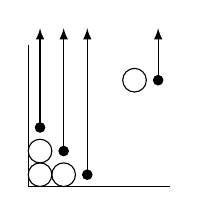
\begin{tikzpicture}[scale=0.3]
\def\rows{6} %number of rows
\def\cols{6} %number of columns
  \draw[-](0,0) -- (\rows,0); %axes
  \draw[-](0,0) -- (0,\cols); 
  \foreach \x/\y in {1/3,2/2,3/1,6/5} { %dot positions
    \draw[fill=black] (\x-0.5,\y-0.5) circle(0.2);
  %line positions
    \draw[-latex](\x-0.5,\y-0.5) -- (\x-0.5,6.7); }
  \foreach \x/\y in {1/1,1/2,2/1,5/5} %circle positions
    \draw (\x-0.5,\y-0.5) circle(0.5);
\end{tikzpicture}
  \caption{\label{fig:bad_va}A bubble diagram which satisfies the bubble popping rule, but is not a permutation diagram.}
\end{center}
\end{figure}

\begin{figure}[ht]
  \begin{displaymath}
    \arraycolsep=0.9\cellsize
    \begin{array}{cc}
      \boxtab{ 
        & & \usebox7 \\
        & \usebox7 & \\
        \usebox7 & & \\
        \usebox3 & \usebox3 & \usebox3 & \usebox7 & \\
        & & & \usebox3 & \usebox7 \\\hline } &
      
    \end{array}
  \end{displaymath}
  \caption{\label{fig:bad_dot}A bubble diagram which satisfies the dot condition, but is not a permutation diagram.}
\end{figure}

\begin{figure}[ht]
  \begin{displaymath}
    \arraycolsep=0.9\cellsize
    \begin{array}{c}
      \cirtab{ 
        & & 4 & 5 & \\
        & & 3 \\
        & 2 \\
        & \\\hline}
      
    \end{array}
  \end{displaymath}
    \caption{\label{fig:bad_number}A bubble diagram which satisfies the numbering condition yet is not a permutation diagram.}
\end{figure}